\section{Target system} \label{sec:target}
\subsection{Luquid $D_2$ target system}

\begin{figure}[htbp]
  \centering
  \includegraphics[width=10cm]{pic/experiment/d2-cryo.eps}
  \caption{
    Schematic drawing of the liquid $D_2$ cryostat.
  }
  \label{fig:d2_cryo}
\end{figure}


A side view of the cryostat for the liquid $D_2$ target is shown in Fig\ref{fig:d2_cryo}.
Deuterium is stored 1000$l$ in a tank as gases which is room temperature and 2atm keeping positive pressure after liquefaction for avoiding contamination from other materials.
The $D_2$ gas is fed into the cryostat through the top flange.
Cooling of $D_2$ is performed by the Gifford–McMahon (G–M) refrigerator (Sumitomo Heavy Industries, Ltd., RDK-145D and CSA-71A) built into the cryostat.
The cooling is performed by 2-step.
The cooling power at the first and second stages is 35$W$ at 50K and 1.5$W$ at 4.2K, respectively.
A copper plate is anchored to the first-stage cold head of the G-M refrigerator in inlet pipe for the pre-cooling of the $D_2$.
Another inlet pipe is directly connected through the top flange to the head exchanger for measuring the pressure of the $D_2$ target inside of the heat exchanger.
Since this pipe has a larger conductance, a safety valve that prevents a sudden pressure rise is also connected to it.
The $D_2$ gas is cooled in the heat exchanger where the second stage of the G–M refrigerator is thermally contacted.

\begin{figure}[htbp]
  \begin{tabular}{cc}
    \begin{minipage}{0.7\hsize}
      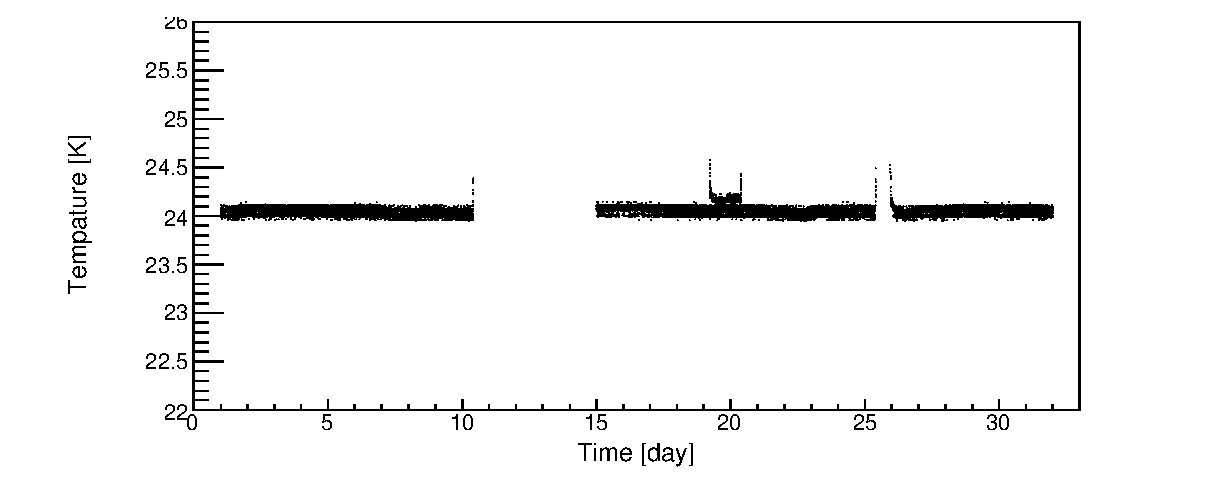
\includegraphics[width=8cm]{../pic/Dron/target/target_temp.eps}
    \end{minipage}
    \begin{minipage}{0.3\hsize}
      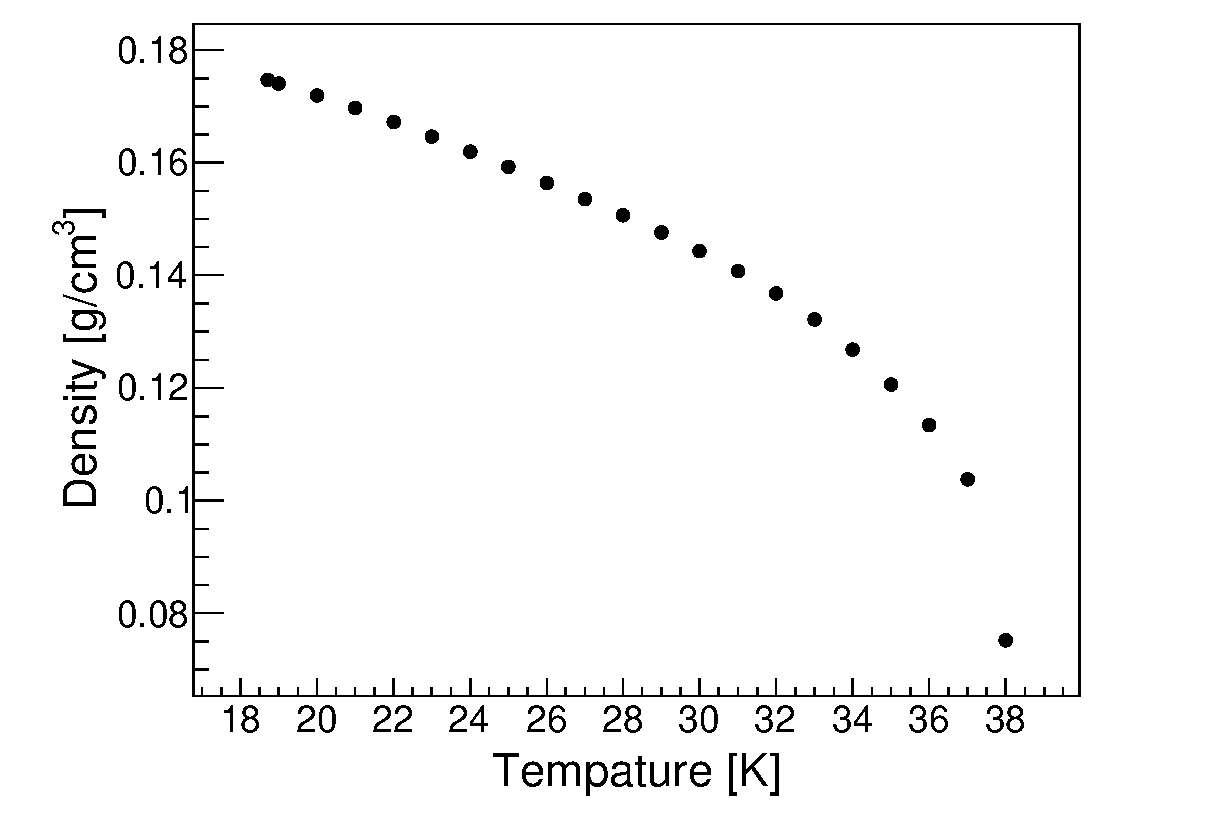
\includegraphics[width=5cm]{../pic/Dron/target/target_den.eps}
    \end{minipage}
  \end{tabular}
  \caption{
    The left figure shows the temperature of the $D_2$ target.
    The right figure shows the relation of the density and the $D_2$ temperature at 1 atm.
  }
  \label{fig:target}
\end{figure}


The target cell is $6.8cm$ diameter and $12.5cm$ length cylinder made of PET.
Liquifregrated $D_2$ is transferred by downpipe and warmed liquid $D_2$ by the heat load is returned through the upper pipe,
so the heat is effectively transferred between the target cell and the heat exchanger\cite{Target}.
Since the temperature range of liquid $D_2$ is narrow as 18.7-23.8K at 1 atm, the temperature of the $D_2$ should be controlled in the liquid range to avoid blocking due to the solid $D_2$.
Since the cooling power of the second stage of the G–M refrigerator is larger than the heat load on the low-temperature parts,
The current in the heater is controlled by a proportional-integral-derivative (PID) algorithm with an input of the temperature of the heat exchanger.
Target cell temperature in MR-RUN78 is represented in Fig\ref{fig:target} which is monitored by Pt-Co thermometer (CHINO R800-6) whose tolerance was $\pm$ 0.5K.
The same figure also shows the relation of temperature and density of $D_2$ at 1 bar.
The error of $D_2$ density was estimated at 1.5$\times 10^{-3} [g/cm^3]$ from tolerance and fluctuation.
